\documentclass[11pt,letterpaper]{article}
\usepackage[margin=2cm]{geometry}
\usepackage{amsmath,amssymb,graphicx,xcolor,booktabs,tabularx,enumitem,titlesec,fancyhdr,array,longtable}
\usepackage{caption}
\usepackage{tikz}
\usetikzlibrary{arrows.meta,positioning,shapes.geometric,calc,decorations.pathmorphing,patterns}
\usepackage[hidelinks]{hyperref}
\usepackage{helvet}\renewcommand{\familydefault}{\sfdefault}
\usepackage{microtype}
\titleformat{\section}{\Large\bfseries\color{blue!50!black}}{\thesection}{0.6em}{}
\titleformat{\subsection}{\large\bfseries}{\thesubsection}{0.6em}{}
\titleformat{\subsubsection}{\normalsize\bfseries}{\thesubsubsection}{0.6em}{}
\setlength{\headheight}{14pt}
\pagestyle{fancy}\fancyhf{}\lhead{sPHENIX Self-Paced Course}\rhead{Module 4: Tracking Detectors}\cfoot{\thepage}
\newcommand{\conceptbox}[2]{\par\medskip\noindent\fcolorbox{blue!50!black}{blue!5}{\begin{minipage}{0.96\linewidth}\textbf{#1}\par\smallskip #2\end{minipage}}\par\medskip}
\newcommand{\connectbox}[1]{\par\medskip\noindent\fcolorbox{green!40!black}{green!5}{\begin{minipage}{0.96\linewidth}\textbf{Connect to your analysis}\par\smallskip #1\end{minipage}}\par\medskip}
\newcommand{\pitfallbox}[1]{\par\medskip\noindent\fcolorbox{red!50!black}{red!4}{\begin{minipage}{0.96\linewidth}\textbf{Pitfalls}\par\smallskip #1\end{minipage}}\par\medskip}
\newcommand{\checksbox}[1]{\par\medskip\noindent\fcolorbox{orange!60!black}{orange!5}{\begin{minipage}{0.96\linewidth}\textbf{Checks}\par\smallskip #1\end{minipage}}\par\medskip}
\newcommand{\workedbox}[2]{\par\medskip\noindent\fcolorbox{gray!60!black}{gray!6}{\begin{minipage}{0.96\linewidth}\textbf{Worked example: #1}\par\smallskip #2\end{minipage}}\par\medskip}
\newcommand{\goal}[1]{\par\noindent\textbf{Goal.} #1\par\smallskip}
\newcommand{\code}[1]{\texttt{#1}}
\setlist{itemsep=1pt,topsep=3pt}
\setlength{\emergencystretch}{3em}
\setlength{\parskip}{3pt}
\captionsetup{font=small}
\begin{document}
\begin{center}{\LARGE\bfseries sPHENIX Self-Paced Course --- Module 4}\\[4pt]
{\Large Tracking detectors: MVTX, INTT, TPC and TPOT}\\[8pt]
Prepared for P.\,D.\ Lewis (Ohio University) \quad November 2026\\[2pt]
\small Self-contained study text built on the Summer-2026 sPHENIX School, public sPHENIX papers and standard detector textbooks\end{center}

\tableofcontents
\newpage

\section*{How to use this module}
\addcontentsline{toc}{section}{How to use this module}
This module is self-contained.
It explains how charged particles are detected in silicon and in gas, and how the four sPHENIX tracking subsystems are built, read out and used.
You do not need slides, recordings or papers to follow it.
The school talks listed below are the \emph{sources}; they are cited as [S\#\#] so that a statement can be traced.
Track reconstruction (seeding, fitting, alignment, TPC distortion corrections) is the subject of Module 8; here we concentrate on the detectors.

\subsection*{Learning objectives}
After this module you should be able to:
\begin{enumerate}[label=O\arabic*.]
\item Explain energy loss of charged particles (Bethe--Bloch, MIP, Landau fluctuations) and multiple Coulomb scattering, and estimate the signal in silicon and in gas.
\item Explain charge collection in a reverse-biased silicon junction, and contrast strips, hybrid pixels and monolithic active pixel sensors (MAPS).
\item Describe the MVTX (ALPIDE MAPS, three layers) and its strobe-based readout, and explain what it contributes to vertex and DCA resolution.
\item Describe the INTT (two barrel layers of silicon strips) and explain why it is the detector that ties tracks to a single bunch crossing.
\item Explain drift, diffusion and gas amplification, and describe the sPHENIX TPC (GEM readout, zigzag pads, continuous readout, ion back-flow, space charge, laser calibration).
\item Describe TPOT (Micromegas) and its role as a distortion-free reference outside the TPC.
\item Compare integration times (MVTX strobe, INTT crossing, TPC drift) and explain the resulting pile-up and timing logic.
\item Relate detector design to momentum and DCA resolution with back-of-the-envelope formulas.
\end{enumerate}

\subsection*{Prerequisites and time}
Modules 1 and 2. Module 3 is helpful but not required.
Estimated time: 9--11 hours (about 6 hours reading, 2 hours worked examples, 1--3 hours optional exercises).

\subsection*{Sources (sPHENIX School 2026, BNL, July 2026)}
\begin{itemize}
\item {[S10]} C. Dean, ``MVTX Overview'' --- silicon physics, MAPS, ALPIDE readout, resolution, vertexing, alignment.
\item {[S11]} A. Enokizono, ``INTT Overview'' --- INTT layout, sensors, readout, timing.
\item {[S12]} T. Hemmick, ``TPC and TPOT Overview'' --- gas detectors, TPC mechanics and physics, space charge, laser calibration, TPOT.
\item {[S28]} T. Kikuchi, ``INTT hit detection efficiency study'' (flash talk) --- how a hit efficiency is measured with tracks.
\end{itemize}

\subsection*{Public readings (optional)}
INTT ladder paper [R1] and beam-test paper [R2]; the INTT detector paper [R3]; sPHENIX TPC design proceedings [R4, R5]; the sPHENIX Au+Au multiplicity paper, which describes the INTT and MVTX as used in a physics result [R6]; the PDG reviews of passage of particles through matter and of particle detectors [R7].

\conceptbox{Notation}{$p_T$ in GeV/$c$, $B$ in tesla, lengths in metres unless stated. ``DCA'' = distance of closest approach of a track to the vertex (also called impact parameter). ``BCO'' = beam-clock counter, i.e.\ a RHIC bunch-crossing number. One RHIC crossing lasts about 106 ns. $X_0$ = radiation length; $x/X_0$ = material thickness in units of $X_0$.}

%=====================================================================
\section{The sPHENIX tracking system at a glance}\label{sec:overview}
\goal{Know which detector sits where, what it measures, and why the system needs all four.}

\subsection{What a tracker must do}
A tracking system has three main tasks [S10]:
\begin{enumerate}
\item record the trajectories of long-lived charged particles (pions, kaons, protons, electrons, muons);
\item find the collision point (primary vertex) and any displaced decay points (secondary vertices);
\item measure momentum and charge from the curvature in the magnetic field.
\end{enumerate}
Secondary tasks are timing (which bunch crossing did a track come from?) and particle identification (from specific energy loss $\mathrm{d}E/\mathrm{d}x$ in gas) [S10].

\subsection{The four subsystems}
\begin{center}\small
\begin{tabularx}{\linewidth}{@{}lllX@{}}\toprule
Detector & Technology & Radius & Main role\\\midrule
MVTX & 3 layers of MAPS pixels (ALPIDE) & $\approx2.5$--4 cm & vertex and DCA precision\\
INTT & 2 layers (4 sub-layers) of Si strips & $\approx7$--10 cm & bunch-crossing timing; links MVTX and TPC\\
TPC & gas TPC, quad-GEM, zigzag pads & $\approx20$--78 cm & momentum, pattern recognition, $\mathrm{d}E/\mathrm{d}x$\\
TPOT & Micromegas, limited $\phi$ coverage & just outside the TPC & distortion-free reference for TPC calibration\\\bottomrule
\end{tabularx}\end{center}
All of them cover roughly $|\eta|<1.1$ (TPOT only partially in $\phi$) inside the 1.4 T solenoid [S10, S11, S12, R4, R6].

\begin{figure}[!htbp]\centering
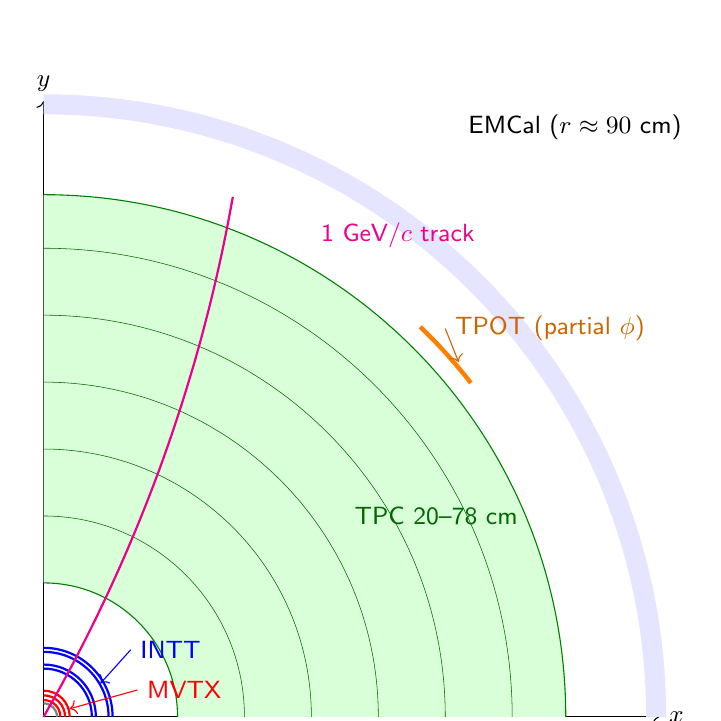
\begin{tikzpicture}[scale=0.085]
% r-phi quarter: radii in cm, scale 0.085 cm per cm
\draw[->] (0,0) -- (92,0) node[right] {\small $x$};
\draw[->] (0,0) -- (0,92) node[above] {\small $y$};
\draw[gray,thick] (0:2) arc (0:90:2);
\foreach \r in {2.5,3.2,3.9} \draw[red,thick] (0:\r) arc (0:90:\r);
\foreach \r in {7.2,7.8,9.7,10.3} \draw[blue,thick] (0:\r) arc (0:90:\r);
\fill[green!15] (0:20) arc (0:90:20) -- (90:78) arc (90:0:78) -- cycle;
\draw[green!50!black] (0:20) arc (0:90:20); \draw[green!50!black] (0:78) arc (0:90:78);
\foreach \r in {30,40,50,60,70} \draw[green!40!black,very thin] (0:\r) arc (0:90:\r);
\draw[orange,ultra thick] (38:81) arc (38:46:81);
\fill[blue!10] (0:90) arc (0:90:90) -- (90:93) arc (90:0:93) -- cycle;
\node[anchor=west,font=\small] at (62,88) {EMCal ($r\approx90$ cm)};
\node[anchor=west,font=\small,green!40!black] at (45,30) {TPC 20--78 cm};
\node[anchor=west,font=\small,orange!80!black] at (60,58) {TPOT (partial $\phi$)};
\draw[->,orange!80!black] (60,58) -- (62,53);
\node[anchor=west,font=\small,red] at (14,4) {MVTX};
\node[anchor=west,font=\small,blue] at (13,10) {INTT};
\draw[->,red] (14,4) -- (3.9,1.2);
\draw[->,blue] (13,10) -- (8.5,5);
% 1 GeV track (R=238 cm): circle through origin, center at (238,0) rotated: param
\draw[thick,magenta,domain=0:20,samples=40] plot ({238*sin(\x)*cos(60)-238*(1-cos(\x))*sin(60)},{238*sin(\x)*sin(60)+238*(1-cos(\x))*cos(60)});
\node[magenta,font=\small,anchor=west] at (40,72) {1 GeV/$c$ track};
\end{tikzpicture}
\caption{Schematic quarter view in the transverse ($r$--$\phi$) plane, radii to scale (silicon layers drawn at approximate radii). The magenta curve is a toy $p_T=1$ GeV/$c$ track in 1.4 T (radius of curvature 2.4 m). TPOT is drawn schematically. Not an event display.}\label{fig:layout}
\end{figure}

\subsection{Why four detectors?}
Each technology is good at something different:
\begin{itemize}
\item \textbf{MVTX} is very close to the beam and very thin, so it gives the best pointing to the vertex. It is slow (microsecond integration).
\item \textbf{INTT} is fast: it records which 106 ns crossing a hit belongs to. It is coarse along $z$.
\item \textbf{TPC} gives many points (48 pad rows) over a long lever arm, which is what measures momentum. It is very slow (about 13 $\mu$s maximum drift) and its points are displaced by drift distortions.
\item \textbf{TPOT} measures points just outside the TPC with negligible drift, which lets the TPC distortions be measured from outside [S12].
\end{itemize}
The combination is a ``timing sandwich'': the silicon detectors tell the TPC which crossing a track belongs to and where it started; the TPC supplies momentum; the silicon and TPOT together constrain the TPC distortions.

\subsection{Layer numbering in software}
In the sPHENIX tracking geometry, the layers are numbered from the inside out: MVTX layers 0--2, INTT layers 3--6, TPC layers 7--54 and TPOT layers 55--56 (check the current coresoftware geometry for any change). You will see these numbers in cluster keys and in residual plots.

\connectbox{Your $\pi^0$/$\eta$ analysis uses the MBD vertex. The tracking system can provide a vertex too, with much better $z$ resolution, but only in events with enough tracks, and only for the crossing that the silicon identifies. Two practical links: (1) your photon candidates can be vetoed against tracks (a cluster matched to a track is a charged particle, not a photon); (2) the material of the trackers converts photons into $e^+e^-$ pairs before they reach the EMCal (Section~\ref{sec:roles}).}

%=====================================================================
\section{Charged particles in matter}\label{sec:dedx}
\goal{Be able to estimate how much charge a minimum-ionising particle leaves in silicon and in gas, how much it scatters, and how it bends.}

\subsection{Energy loss: the Bethe--Bloch formula}
A charged particle passing through matter loses energy mainly by kicking atomic electrons.
A short classical argument gives the scaling [S10].
An electron at impact parameter $b$ receives a momentum kick $\Delta p=\int F\,\mathrm{d}t=2ze^2/(bv)$ (Gauss's law for a straight-line passage at speed $v$).
Its energy gain is $\Delta E=\Delta p^2/2m_e\propto z^2/(b^2v^2)$.
Integrating over electrons in a shell $2\pi b\,\mathrm{d}b\,\mathrm{d}x$ between $b_{\min}$ and $b_{\max}$ gives a logarithm of $b_{\max}/b_{\min}$.
The full relativistic quantum result is the Bethe--Bloch formula [R7]:
\begin{equation}
-\Big\langle\frac{\mathrm{d}E}{\mathrm{d}x}\Big\rangle=K z^2\frac{Z}{A}\frac{1}{\beta^2}\left[\frac12\ln\frac{2m_ec^2\beta^2\gamma^2T_{\max}}{I^2}-\beta^2-\frac{\delta(\beta\gamma)}{2}\right],\qquad K\approx0.307\ \mathrm{MeV\,cm^2/mol}.
\end{equation}
Its shape is what matters:
\begin{itemize}
\item at low momentum the $1/\beta^2$ term dominates, so slow particles lose much more energy;
\item there is a broad minimum near $\beta\gamma\approx3$--4: a particle there is a \emph{minimum-ionising particle} (MIP);
\item above it the loss rises slowly (relativistic rise), tamed by the density effect $\delta$.
\end{itemize}
At fixed momentum, heavier particles have smaller $\beta$, so protons and kaons at $p<1$ GeV/$c$ ionise much more than pions. This is the basis of $\mathrm{d}E/\mathrm{d}x$ particle identification in the TPC.

\subsection{Fluctuations: the Landau distribution}
The energy lost in a thin layer fluctuates strongly, because rare hard collisions (producing energetic ``delta electrons'') carry a lot of energy.
The distribution is asymmetric, with a long tail to high energy (Landau--Vavilov distribution).
The most probable value (MPV) is noticeably below the mean.
For a thin layer it is better to quote the MPV, and for $\mathrm{d}E/\mathrm{d}x$ in a TPC one uses a \emph{truncated mean} (drop the highest samples) to suppress the tail.

\workedbox{charge from a MIP in silicon}{For silicon, $\langle\mathrm{d}E/\mathrm{d}x\rangle_{\min}\approx1.66$ MeV\,cm$^2$/g $\times\,2.33$ g/cm$^3\approx3.9$ MeV/cm $=390$ eV/$\mu$m. Creating one electron--hole pair costs 3.6 eV. So the mean is about $390/3.6\approx108$ pairs per $\mu$m; the most probable value is lower, roughly 70--80 pairs per $\mu$m for thin sensors [S10, R7].\\[2pt]
\textbf{INTT} (320 $\mu$m): mean $\approx3.4\times10^4$ electrons, MPV $\approx2.4\times10^4$. Easy to see above electronic noise of order $10^3$ electrons.\\
\textbf{MVTX}: the charge is collected mostly from a thin (tens of $\mu$m) high-resistivity epitaxial layer, so a MIP gives of order $10^3$ electrons, shared over a few pixels. The pixel threshold is of order 100 electrons [S10], well below this.}

\workedbox{electrons per cm in TPC gas}{Typical total ionisation for a MIP (PDG table): neon $\approx39$ electrons/cm, CF$_4\approx100$/cm, argon $\approx94$/cm, isobutane $\approx195$/cm [R7]. A Ne:CF$_4$ 50:50 mixture gives about 70 electrons/cm; an Ar:CF$_4$:iC$_4$H$_{10}$ 75:20:5 mixture about 100/cm. A pad row about 1 cm long collects therefore of order 100 electrons in many small clusters. This is too little to read directly, so the TPC needs gas amplification of order $10^3$ (Section~\ref{sec:gas}).}

\subsection{Multiple Coulomb scattering}
A charged particle also scatters elastically off nuclei.
The net deflection after a layer of thickness $x$ is roughly Gaussian with width [R7]
\begin{equation}
\theta_0=\frac{13.6\ \mathrm{MeV}}{\beta cp}\,z\sqrt{\frac{x}{X_0}}\left[1+0.038\ln\frac{x z^2}{X_0\beta^2}\right].
\end{equation}
It scales as $1/p$ and as $\sqrt{x/X_0}$.
At low momentum it dominates the track pointing resolution; this is why vertex detectors must be thin and close to the beam.

\workedbox{scattering in the beam pipe and first MVTX layer}{Take $x/X_0\approx0.5\%$ for the beam pipe plus one MVTX layer (each MVTX layer is about 0.3\% $X_0$ [S10]). For $p=1$ GeV/$c$: $\theta_0=13.6\times10^{-3}\times\sqrt{0.005}\times[1+0.038\ln0.005]\approx0.77$ mrad. Projected over the distance to the first layer, $r_1\approx2.5$ cm, this gives about $2.5\ \mathrm{cm}\times0.77\ \mathrm{mrad}\approx19\ \mu$m. At 0.5 GeV/$c$ it is about 38 $\mu$m; at 5 GeV/$c$ about 4 $\mu$m. Compare the MVTX hit resolution of a few $\mu$m [S10]: below a few GeV/$c$ scattering, not pixel size, limits the DCA resolution. (Estimate.)}

\subsection{Motion in a magnetic field}
In a solenoidal field $B$ along $z$, a particle moves on a helix.
Its transverse radius of curvature is
\begin{equation}
R\,[\mathrm{m}]=\frac{p_T\,[\mathrm{GeV}/c]}{0.3\,B\,[\mathrm{T}]}.
\end{equation}
In 1.4 T a 1 GeV/$c$ track has $R=2.38$ m; a 0.3 GeV/$c$ track has $R=0.71$ m.
A track from the origin reaches radius $r$ at an azimuthal deviation $\Delta\phi=\arcsin(r/2R)$ from its initial direction.
Very soft tracks ($p_T\lesssim0.15$ GeV/$c$, $2R<0.78$ m) curl up inside the TPC (``loopers'') [S10].
Positive and negative particles bend in opposite directions.

\workedbox{a 1 GeV/$c$ pion through the tracker (checkpoint exercise)}{With $R=2.38$ m, $\Delta\phi(r)=\arcsin(r/4.76\ \mathrm{m})$:
\begin{center}\small\begin{tabular}{@{}lcccccc@{}}\toprule
Layer & MVTX 2.5 & MVTX 3.9 & INTT 7.2 & INTT 10.3 & TPC 20 & TPC 78 cm\\\midrule
$\Delta\phi$ (deg) & 0.30 & 0.47 & 0.87 & 1.24 & 2.41 & 9.43\\\bottomrule
\end{tabular}\end{center}
The silicon hits lie almost on a straight line; the curvature is measured over the TPC. The sagitta over the TPC chord (about 0.58 m) is $s\approx L^2/8R=1.8$ cm. A 5 GeV/$c$ track has a sagitta of only 3.5 mm, which is why momentum resolution degrades with $p_T$. Expect 3 MVTX hits, 2 INTT hits (one in each barrel, from one of the two staggered sub-layers), up to 48 TPC clusters, and a TPOT hit only if the track points into a TPOT module.}

%=====================================================================
\section{Silicon detectors: from the pn junction to MAPS}\label{sec:si}
\goal{Understand how a silicon sensor turns ionisation into a signal, and why strips, hybrid pixels and MAPS make different trade-offs.}

\subsection{The reverse-biased junction}
Pure silicon has four valence electrons.
Doping with a five-valence element (e.g.\ phosphorus) gives n-type material with free electrons (donors); doping with a three-valence element (e.g.\ boron) gives p-type material with free holes (acceptors) [S10].
At a pn junction, carriers diffuse across and recombine, leaving a \emph{depletion zone} free of mobile charge, with a built-in electric field.
A reverse bias (positive on the n side) widens the depletion zone.
In a fully depleted sensor, an ionising particle creates electron--hole pairs which drift in the field to the electrodes; their motion induces the signal.
The depletion width for a bias $V$ is approximately [S10]
\begin{equation}
W(V)\approx\sqrt{\frac{2\varepsilon_0\varepsilon_{\rm Si}V}{eN_D}}=\sqrt{2\varepsilon_0\varepsilon_{\rm Si}\,\mu\,\rho\,V},
\end{equation}
with $N_D$ the dopant concentration, $\rho$ the resistivity and $\mu$ the carrier mobility.

\workedbox{depletion widths}{With $\rho=20$ k$\Omega$\,cm and $\mu=1350$ cm$^2$/(V\,s): $W(1\ \mathrm{V})\approx75\ \mu$m and $W(45\ \mathrm{V})\approx500\ \mu$m. Because $W\propto\sqrt{V}$, doubling the depleted thickness needs four times the voltage. Thick strip sensors need tens to hundreds of volts; MAPS with a thin sensitive layer need only a few volts [S10].}

\subsection{Three silicon technologies}
\begin{itemize}
\item \textbf{Strips.} Long, narrow electrodes (pitch 20--100 $\mu$m, length of cm). One coordinate is measured precisely, the other only to the strip length. Mature, cheap, reliable to manufacture [S10].
\item \textbf{Hybrid pixels.} A pixelated sensor bump-bonded pixel by pixel to a readout chip. Two precise coordinates, fast, but bump bonding is delicate and adds material [S10].
\item \textbf{Monolithic active pixel sensors (MAPS).} Sensor and readout electronics in the same CMOS chip; no bump bonds. Pixels can be small (20--30 $\mu$m), the chip can be thinned to tens of $\mu$m, and power is low. The price is speed (microsecond integration) [S10].
\end{itemize}

\begin{center}\small
\begin{tabularx}{\linewidth}{@{}lXXXX@{}}\toprule
 & Cell size & Speed & Thickness & Bias, power\\\midrule
Strips & 20--100 $\mu$m $\times$ cm & fast & few hundred $\mu$m & high (100--500 V), high power\\
Hybrid pixels & 50--100 $\mu$m & fast & few hundred $\mu$m & high, high power\\
MAPS & 20--100 $\mu$m & slow ($\mu$s) & tens of $\mu$m & low (few V), low power\\\bottomrule
\end{tabularx}\end{center}
(Qualitative comparison following [S10].)

\subsection{Position resolution of a binary cell}
If a detector only says ``hit'' or ``no hit'' for a cell of pitch $p$, and a particle hits anywhere in the cell with flat probability, the rms error is [S10]
\begin{equation}
\sigma^2=\frac1p\int_{-p/2}^{p/2}x^2\,\mathrm{d}x=\frac{p^2}{12},\qquad\sigma=\frac{p}{\sqrt{12}}.
\end{equation}
For the MVTX pixel ($\approx29\ \mu$m) this gives about 8 $\mu$m; for the INTT strip pitch (78 $\mu$m) about 23 $\mu$m; along the INTT strip length (16 or 20 mm) about 4.6--5.8 mm.
When charge is shared between neighbouring cells, the centroid of the cluster is more precise than $p/\sqrt{12}$; this is why multi-pixel clusters improve the resolution [S10]. The MVTX reaches a hit resolution of a few $\mu$m this way [S10].

\subsection{Clustering}
A particle usually fires more than one cell: it may cross a cell boundary, enter at an angle, or the charge diffuses.
Clustering groups adjacent fired cells.
It is naturally formulated as finding connected components of a graph whose nodes are fired cells and whose edges join neighbours [S10].
Hot (always-on) cells create fake clusters or bias real ones; dead cells split clusters; both must be masked [S10].
Clusters are larger for tracks at large $|\eta|$, which cross the sensor at a shallow angle and so traverse more silicon [S10].

\subsection{Radiation damage}
Radiation damages silicon by displacing lattice atoms (vacancies and interstitials, described by the non-ionising energy loss) and by ionisation in the oxide layers [S10].
The consequences are higher leakage current, lower charge-collection efficiency, and (for thick sensors) a change of the depletion voltage.
For MAPS, damage and environment shift the effective threshold and noise of the pixels, which are therefore monitored over time and re-tuned [S10].

%=====================================================================
\section{The MVTX}\label{sec:mvtx}
\goal{Know the MVTX layout and ALPIDE readout well enough to explain its integration time, its noise masking, and its contribution to the DCA.}

\subsection{Layout and the ALPIDE chip}
The MVTX has three layers of MAPS staves, at radii from about 2.5 cm to 4 cm, built on the ALICE ITS2 inner-barrel design [S10].
It uses the ALPIDE chip (ALice PIxel DEtector) [S10]:
\begin{center}\small
\begin{tabular}{@{}ll@{}}\toprule
Technology & 180 nm CMOS MAPS\\
Sensor thickness & 50 $\mu$m\\
Pixel size & $\approx29\times27\ \mu$m$^2$\\
Matrix & $1024\times512$ pixels per chip\\
Material per layer (stave) & $\approx0.3\%\,X_0$\\
Hit resolution & a few $\mu$m\\
Integration (strobe) time & several $\mu$s\\
Total channels & $\approx226$ million pixels\\\bottomrule
\end{tabular}\end{center}
(Design specifications as presented in [S10].)
The front-end readout uses the ALICE Readout Unit, and the back end uses FELIX boards developed for ATLAS [S10].
The innermost layer sits only about 2.5 cm from the beam line, just outside the beryllium section of the beam pipe [S10].

\subsection{How a pixel records a hit}
Each pixel has an in-pixel amplifier and discriminator.
When the collected charge exceeds the threshold (of order 100 electrons [S10]), the discriminator output goes high for a time that depends on the charge (microseconds).
The chip latches a hit only if this output overlaps a \textbf{strobe} window [S10].
There are three ways to operate:
\begin{itemize}
\item \textbf{Streaming mode:} strobes are issued continuously, back to back (windows of order 10 $\mu$s with a short gap). Every hit overlaps some strobe and is recorded [S10].
\item \textbf{Triggered mode:} a short strobe is issued only after a trigger. Because the trigger arrives a few $\mu$s after the collision (latency), the hit is recorded only if the discriminator is still high when the strobe arrives [S10].
\item \textbf{Extended (triggered) mode:} a long strobe is opened on a trigger, giving the robustness of streaming within a window [S10].
\end{itemize}

\begin{figure}[!htbp]\centering
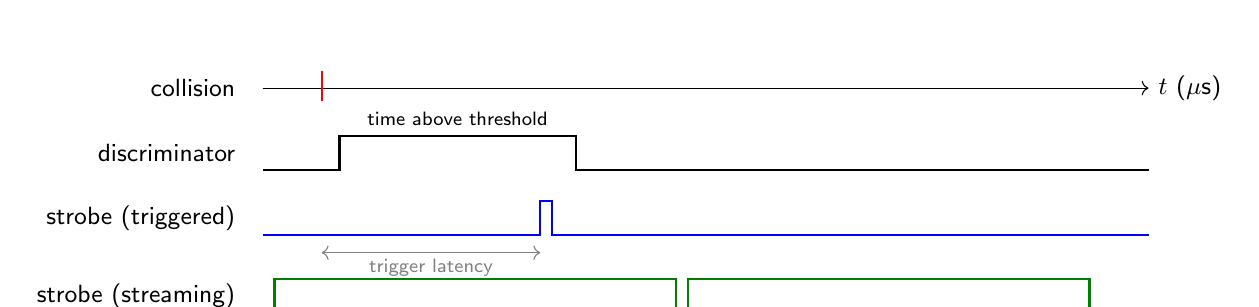
\begin{tikzpicture}[xscale=0.75,yscale=0.55]
\node[anchor=east,font=\small] at (-0.3,4.5) {collision};
\draw[->] (0,4.5) -- (15,4.5) node[right,font=\small] {$t$ ($\mu$s)};
\draw[red,thick] (1,4.2) -- (1,4.9);
\node[anchor=east,font=\small] at (-0.3,3) {discriminator};
\draw[thick] (0,2.6) -- (1.3,2.6) -- (1.3,3.4) -- (5.3,3.4) -- (5.3,2.6) -- (15,2.6);
\node[font=\scriptsize] at (3.3,3.8) {time above threshold};
\node[anchor=east,font=\small] at (-0.3,1.5) {strobe (triggered)};
\draw[thick,blue] (0,1.1) -- (4.7,1.1) -- (4.7,1.9) -- (4.9,1.9) -- (4.9,1.1) -- (15,1.1);
\draw[<->,gray] (1,0.7) -- (4.7,0.7); \node[font=\scriptsize,gray] at (2.85,0.35) {trigger latency};
\node[anchor=east,font=\small] at (-0.3,-0.3) {strobe (streaming)};
\draw[thick,green!50!black] (0,-0.7) -- (0.2,-0.7) -- (0.2,0.1) -- (7.0,0.1) -- (7.0,-0.7) -- (7.2,-0.7) -- (7.2,0.1) -- (14,0.1) -- (14,-0.7) -- (15,-0.7);
\end{tikzpicture}
\caption{Schematic ALPIDE timing (toy durations). A hit is latched if the discriminator output overlaps a strobe. In triggered mode a short strobe arrives after the trigger latency; if the discriminator has already returned low, the hit is lost. In streaming mode back-to-back strobes always overlap.}\label{fig:strobe}
\end{figure}

\pitfallbox{In triggered mode, hits whose discriminator pulse is shorter than the trigger latency are lost. The time above threshold depends on the deposited charge, so the loss is not uniform: it can depend on particle type, momentum and $\eta$ (large-$|\eta|$ tracks cross more silicon; slow, heavily ionising particles deposit much more charge) [S10]. An efficiency measured in streaming mode does not automatically apply to triggered data.}

\subsection{Data reduction}
The MVTX is binary: each pixel is on or off; no amplitude is stored [S10].
Only fired pixels are sent (zero suppression).
In a typical event only a tiny fraction of the pixels fire, of order $10^{-4}$ [S10].
The address encoding is optimised: with 512 rows and 1024 columns, a pixel address needs $9+10=19$ bits.
Eight hits would need 152 bits if sent one by one, but if one sends the first address and then a small bitmap of which neighbours are also hit, a cluster of 8 pixels costs only a few tens of bits [S10].

\subsection{Noisy pixels and masking}
Because all signals look the same (a fired pixel), a few stuck or noisy pixels per chip can produce as many hits as real particles [S10].
In a chip with half a million pixels and a few tens of real hits per event, a couple of dozen permanently-on pixels would hide the signal.
Noisy pixels are therefore identified in dedicated runs and masked [S10].
Their number changes with time (radiation, settings), so masks are part of the conditions.

\subsection{Impact-parameter resolution}
A useful approximation for the DCA resolution of a two-layer telescope is
\begin{equation}
\sigma_{\rm DCA}^2\approx\sigma_{\rm geom}^2+\left(\frac{r_1\cdot13.6\ \mathrm{MeV}}{p_T\,c}\sqrt{\frac{x}{X_0}}\left[1+0.038\ln\frac{x}{X_0}\right]\right)^2,
\end{equation}
where $\sigma_{\rm geom}$ depends on the hit resolutions and the lever arm between layers, $r_1$ is the radius of the first measurement and $x/X_0$ the material before it [S10].
Both terms favour small $r_1$ and little material: hence the MVTX at 2.5 cm with 0.3\% $X_0$ per layer.
From the earlier worked example the scattering term is about 20 $\mu$m at 1 GeV/$c$, so the MVTX DCA resolution at low $p_T$ is set by scattering.
This DCA precision is what allows heavy-flavour hadrons (with $c\tau$ of order 100--500 $\mu$m) to be separated from prompt particles.

\subsection{Vertexing with the MVTX}
Once tracks exist, the primary vertex is found by extrapolating them back and finding where they meet [S10].
The beam spot is small and stable in $x$--$y$ (order 100 $\mu$m) but long in $z$ (tens of cm) [S10].
A standard procedure: fit a vertex; remove tracks that are obviously incompatible (large DCA); test the effect of removing each track in turn on the vertex $\chi^2$, and drop tracks that change it most. This rejects tracks from displaced decays [S10].

\subsection{Alignment}
Mechanical survey (coordinate-measuring machines, laser scans) gives positions to some tens of $\mu$m, but the detector moves when the magnet is on or when it warms up by 10--20 K during operation [S10].
Cosmic rays (straight tracks, especially with the field off) and dedicated early-run data are used to align the sensors in situ [S10].
Alignment procedures are treated in Module 8.

\checksbox{\begin{itemize}
\item Chip hit maps: after masking, the occupancy should be smooth; isolated very high bins are noisy pixels.
\item Cluster size vs.\ $\eta$: should increase with $|\eta|$ [S10].
\item Threshold and noise per layer versus time: drifts indicate radiation effects or settings changes [S10].
\item Strobe/BCO bookkeeping: in streaming data, check which strobe a hit belongs to before associating it with a trigger.
\end{itemize}}

%=====================================================================
\section{The INTT}\label{sec:intt}
\goal{Know the INTT layout and readout, and understand why its single-crossing timing is the key to using the slow MVTX and TPC data.}

\subsection{Layout}
The INTT is a two-layer barrel of silicon strip ladders covering the full azimuth and $|\eta|<1.1$, between the MVTX and the TPC [S11, R1, R6].
\begin{itemize}
\item 56 ladders: 24 in the inner barrel, 32 in the outer barrel [S11].
\item Each barrel consists of two staggered sub-layers, so that the gaps of one are covered by the other; the four sub-layer radii are about 7.2, 7.8, 9.7 and 10.3 cm [S11].
\item Sensors are 320 $\mu$m thick with 78 $\mu$m strip pitch [S11, R1].
\item Two sensor types along $z$: type A with 16 mm strips and type B with 20 mm strips [S11, R1].
\item Strips run along $z$, so the INTT measures $r\phi$ precisely ($\approx23\ \mu$m binary) and $z$ only to the strip length.
\end{itemize}
Small longitudinal gaps come from the inactive edges of the sensors, and small azimuthal gaps from the two detector halves not closing perfectly [S11].

\subsection{Channels and readout}
Each half-ladder carries one type-A and one type-B sensor and is read by FPHX chips, one per block of 128 strips; the FPHX chip and much of the design come from the PHENIX FVTX [S11, R1].
Counting [S11]:
\begin{itemize}
\item type A: $128\times16=2048$ channels; type B: $128\times10=1280$; so 3328 channels per half-ladder;
\item 112 half-ladders, so $3328\times112=372\,736$ channels in total.
\end{itemize}
The signal path is: sensor $\to$ FPHX on the high-density interconnect (HDI) $\to$ bus extender and conversion cable $\to$ readout card (ROC, re-used from PHENIX FVTX) $\to$ FELIX servers in the counting house [S11, R1].
There are 16 ROCs (8 north, 8 south) and 8 FELIX servers [S11].
The FPHX provides a hit with a coarse amplitude (a few-bit ADC) and its beam-crossing number [R1].

\subsection{Timing: one crossing}
The INTT readout records each hit with the granularity of one RHIC crossing (106 ns) [R3].
Its intrinsic time resolution is much better than the crossing spacing, so after the timing is tuned in commissioning (a delay scan in steps of a fraction of a crossing), essentially all hits from a collision fall into one crossing [S11, R3].
This makes the INTT the detector that assigns a track to its bunch crossing [R2, R3].

\subsection{Triggered and streaming operation}
The FELIX-based readout can run triggered or streaming [S11]:
\begin{itemize}
\item \textbf{Triggered (extended)} readout, used in Au+Au and part of $p$+$p$: on a trigger, hits are read for a window of about 100 crossings (about 10 $\mu$s) [S11].
\item \textbf{Streaming} readout, used in $p$+$p$ and O+O: hits are recorded continuously; the crossing counter of the FPHX is reset every RHIC revolution at the abort gap, so a ``strobe'' covers one turn of the beam [S11].
\end{itemize}

\subsection{Performance checks with physics}
\begin{itemize}
\item \textbf{Good-channel selection:} hot, cold and dead channels are identified in data and removed; in the public Au+Au multiplicity analysis they were about 4\% of the channels [R6].
\item \textbf{Synchronisation:} the numbers of clusters in the inner and outer layers must be correlated event by event; so must the INTT cluster count and the MBD charge sum. A broken correlation reveals desynchronised servers or subsystems [S11].
\item \textbf{Vertex:} the INTT $z$ vertex (from tracklets) correlates with the MBD $z$ vertex; the transverse beam position varies with $z$ because of the beam crossing angle [S11].
\item \textbf{Hit efficiency:} the public beam test found a signal-to-noise ratio above 15 and a hit efficiency above 99\% [R2]; the installed detector reproduces this [R3].
\end{itemize}

\subsection{How a hit efficiency is measured (method)}
The flash talk [S28] illustrates a general method that you can reuse for any layer:
\begin{enumerate}
\item Choose a \emph{target} layer (here the inner INTT). Reconstruct tracks \emph{without} it (MVTX triplet + outer INTT).
\item Select clean tracks: a good primary vertex (several tracks), small DCA, isolation from other tracks, unshared clusters.
\item Project each track to the target layer. Keep only projections inside the fiducial area (away from chip edges, dead or hot channels).
\item Search for a cluster within a residual window (only in $\phi$, because the $z$ resolution is coarse) and in the right time bucket.
\item Efficiency = (tracks with a matched cluster) / (tracks projected into the fiducial area), per half-ladder.
\end{enumerate}
The method measures the \emph{hit} efficiency of the active area, not tracking efficiency or acceptance.
Two subtleties: an impure track sample biases the efficiency low; and hits can leak into the neighbouring crossing or be ``carried over'' from the previous turn, so the time-bucket choice matters [S28].

\connectbox{The same tag-and-probe logic appears in your analysis: the trigger efficiency of the Photon trigger is measured on events taken with an independent (minimum-bias) trigger, and your single-photon efficiency is defined relative to a clean reference. In each case: define the probe sample independently of the thing you measure; restrict to a fiducial region; and check purity.}

\pitfallbox{\begin{itemize}
\item The INTT $z$ coordinate is only known to the strip length (16 or 20 mm). Do not expect mm-level $z$ from INTT-only tracklets; the vertex $z$ resolution comes from combining many tracklets.
\item Do not compare INTT occupancies across runs without the good-channel map for each run.
\item In streaming data, hits from neighbouring crossings are present; a cut on the crossing number relative to the trigger is required.
\end{itemize}}

%=====================================================================
\section{Gas detectors: drift, diffusion and amplification}\label{sec:gas}
\goal{Understand the physics that sets the TPC's precision and its main difficulty, space charge.}

\subsection{From wire chambers to micro-pattern detectors}
In a gas detector, a charged particle ionises gas atoms; the freed electrons drift in an electric field to a region of very high field where they multiply in an avalanche, producing a measurable signal [S12].
\begin{itemize}
\item In a \textbf{Geiger--M\"uller} tube the avalanche runs away (photons from the avalanche ionise elsewhere): a large signal, but independent of the deposited energy and with long dead time [S12].
\item Adding a \textbf{quencher} (a polyatomic gas that absorbs energy in vibrations and rotations) breaks the feedback loop and gives a \textbf{proportional} signal [S12].
\item Multi-wire proportional chambers and drift chambers measure positions with arrays of wires; the \textbf{TPC} drifts the charge over a long distance to a segmented readout plane and measures the third coordinate from the drift time [S12].
\item Modern amplification stages are micro-pattern gas detectors (MPGDs): \textbf{GEMs} (thin perforated foils with a high field in the holes) and \textbf{Micromegas} (a micro-mesh above the pads with a very narrow, high-field gap) [S12].
\end{itemize}

\subsection{Drift}
In a field $\vec E$, electrons reach a constant drift velocity $v_d$, set by collisions with gas molecules.
With a magnetic field $\vec B$, the Langevin equation gives
\begin{equation}
\vec v_d=\frac{\mu E}{1+\omega^2\tau^2}\left[\hat E+\omega\tau\,\hat E\times\hat B+\omega^2\tau^2(\hat E\cdot\hat B)\hat B\right],\qquad\omega=\frac{eB}{m_e},
\end{equation}
where $\tau$ is the mean time between collisions and $\mu=e\tau/m_e$ the mobility.
If $\vec E\parallel\vec B$ (the ideal TPC), the drift is straight along the field lines.
Any component of $\vec E$ perpendicular to $\vec B$ (from field-cage imperfections, the field of accumulated ions, or non-uniformity of $\vec B$) makes the electrons drift sideways (``$E\times B$ distortion'').
The sPHENIX gas has a high drift velocity, about 8 cm/$\mu$s in the Ne:CF$_4$ design mixture [R5].

\subsection{Diffusion}
A drifting electron cloud spreads by diffusion: $\sigma=D\sqrt{L}$ for drift length $L$, with $D$ the diffusion coefficient (in $\mu$m/$\sqrt{\mathrm{cm}}$).
A magnetic field parallel to $\vec E$ reduces the \emph{transverse} diffusion by a factor of about $1/\sqrt{1+\omega^2\tau^2}$, because electrons spiral around the field lines.
CF$_4$ mixtures combine a high drift velocity with a large $\omega\tau$, hence low transverse diffusion in 1.4 T [R4, R5].
Low diffusion is good for resolution, but if the cloud becomes narrower than a pad, most hits land on a single pad and the position information is lost; this is why sPHENIX uses \textbf{zigzag pads} that share charge between neighbours (Section~\ref{sec:tpc}) [S12].

\subsection{Gas amplification}
In a high field, an electron gains enough energy between collisions to ionise; the number of electrons grows as $\mathrm{d}N=\alpha N\,\mathrm{d}x$ (Townsend coefficient $\alpha$), so the gain is $G=\exp\!\int\alpha\,\mathrm{d}x$.
A stack of several GEM foils shares the gain among stages, which makes operation stable (lower sparking risk) and allows the ion back-flow to be minimised [S12].

\subsection{Ion back-flow and space charge}
Each avalanche produces as many positive ions as electrons.
Ions are about a thousand times slower than electrons.
If they flow back into the drift volume (\textbf{ion back-flow}, IBF), they accumulate and distort the drift field [S12].
The ion density in the drift volume comes from two sources: primary ionisation from tracks, and back-flowing ions from the amplification.

\workedbox{why IBF must be below about 1\%}{Let $n_p$ be the primary electrons per unit time. The back-flowing ions per unit time are $n_p\times G\times\epsilon_{\rm IBF}$. With $G=2000$ and $\epsilon_{\rm IBF}=1\%$, each primary electron sends back 20 ions: the back-flow is 20 times the primary ionisation. With $\epsilon_{\rm IBF}=0.2\%$ it is 4 times. Ions drift slowly: with a toy mobility of 2--4 cm$^2$/(V\,s) in a 400 V/cm field they move 8--16 m/s, so they need of order 0.1 s to cross 1 m. At a collision rate of tens of kHz, the ions of thousands of events are in the volume at any time. The distortion is therefore set by the average luminosity and the IBF, and it fluctuates with the beam. (Toy numbers.)}

The sPHENIX TPC uses a quadruple-GEM stack operated in a low-IBF configuration (following the ALICE TPC upgrade), with an IBF of order 1\% or below [S12, R4, R5].
Because the drift field is ungated (no gating grid closes after each event), the TPC can read continuously [R5].

\subsection{Gas choice}
The design gas was Ne:CF$_4$, chosen for high drift velocity, low transverse diffusion and fast ion drift [R4, R5].
Different Ne:CF$_4$ ratios trade diffusion against electron attachment (loss of drifting electrons to CF$_4$ in high-field regions) [S12].
When the war in Ukraine disrupted the world neon supply and its price rose sharply, the collaboration re-optimised the gas and settled on an argon-based mixture, Ar:CF$_4$:isobutane (75:20:5), which mimics the Ne:CF$_4$ properties and proved robust against discharges from highly ionising particles [S12].

%=====================================================================
\section{The sPHENIX TPC}\label{sec:tpc}
\goal{Know the TPC geometry, readout and calibration tools, and how its design sets momentum resolution and pile-up.}

\subsection{Design philosophy}
The TPC is the main tracker and provides the momentum resolution [S12].
Three design principles [S12]:
\begin{enumerate}
\item \textbf{Large lever arm:} maximise the active radial range, so make the field cages as thin as possible.
\item \textbf{High precision:} good single-point resolution from a low-diffusion gas and charge-sharing zigzag pads.
\item \textbf{High accuracy:} low distortions, from low IBF and from calibration tools (lasers, and silicon and TPOT as external references).
\end{enumerate}

\subsection{Geometry and mechanics}
\begin{itemize}
\item Active radius about 20 to 78 cm, $|\eta|<1.1$; the outer radius is smaller than the inner radius of the ALICE TPC [R4, R5].
\item A central membrane at $z=0$ at high voltage divides the TPC into two halves; electrons drift about 1.05 m to each endcap in a field of about 400 V/cm [R4, R5].
\item The maximum drift time is $105\ \mathrm{cm}/(8\ \mathrm{cm}/\mu\mathrm{s})\approx13\ \mu$s.
\item Each endcap (``wagon wheel'', one piece of aluminium) holds 12 sectors, each with three radial modules R1, R2, R3, i.e.\ 72 modules in total; each module has 16 pad rows, so there are 48 pad rows (layers) [S12].
\item The field cages are honeycomb/carbon-fibre composites with Kapton insulation and printed field-shaping stripes connected by resistor chains; the stripes make the drift field uniform close to the cage walls [S12].
\item The mechanics were designed to survive a magnet quench (eddy currents, deflections) [S12].
\end{itemize}

\subsection{Readout: GEMs, zigzag pads, SAMPA, FELIX}
\begin{itemize}
\item \textbf{GEM stack.} Four GEM foils per module amplify the drift electrons. The foils are segmented to limit the energy of a discharge [S12].
\item \textbf{Zigzag pads.} The pads under the GEMs interleave like the teeth of two combs; each pad's tips reach deep into the neighbour (``incursion''). With a narrow charge cloud, rectangular pads would often see the charge on one pad only (position known only to $p/\sqrt{12}$); zigzags share the charge and give a resolution that is a small fraction of the pitch. Laboratory studies showed that incursions close to 100\% and very small gaps between pads give the best linearity [S12, R4].
\item \textbf{Front-end.} The signals are shaped and digitised continuously by the SAMPA chip (developed by ALICE), in a version modified for sPHENIX with a faster peaking time [S12, R4, R5]. Each front-end card (FEE) reads 256 pads; a sector is served by roughly two dozen FEEs, i.e.\ of order 600 FEEs for the whole TPC (the exact count is in the TPC documentation) [S12].
\item \textbf{Back-end.} Data aggregation modules (DAMs) based on FELIX boards, one per sector (24 in total), each in an event-buffer and data-compressor (EBDC) server [S12].
\end{itemize}

\subsection{What the TPC measures}
For each cluster the TPC provides $r$ (the pad row), $\phi$ (the charge centroid across pads) and $z$ (from the drift time).
Note that $z$ is measured as $z=z_{\rm end}\mp v_d\,(t-t_0)$: it requires the collision time $t_0$.
The drift velocity $v_d$ must be known everywhere, and $t_0$ must come from another detector.

\workedbox{wrong crossing means wrong $z$}{If a track is assigned to a crossing one bunch too early or too late, $t_0$ is off by 106 ns and all its TPC clusters move by $v_d\times106\ \mathrm{ns}\approx8\ \mathrm{cm}/\mu\mathrm{s}\times0.106\ \mu\mathrm{s}\approx8.5$ mm in $z$ --- in opposite directions on the two sides of the central membrane. A track crossing the membrane then appears broken, and its TPC segment no longer points to the silicon hits. This is why the INTT crossing assignment is essential [S10, S11].}

\subsection{Momentum resolution}
For $N$ equally spaced points with resolution $\sigma_x$ over a lever arm $L$ in a field $B$, the curvature measurement gives (Gluckstern) [R7]
\begin{equation}
\left(\frac{\sigma_{p_T}}{p_T}\right)_{\rm meas}=\frac{\sigma_x\,p_T}{0.3\,B\,L^2}\sqrt{\frac{720}{N+4}},
\end{equation}
and multiple scattering adds a constant term $(\sigma_{p_T}/p_T)_{\rm ms}\approx\frac{0.0136}{0.3BL\beta}\sqrt{x/X_0}\times\mathcal{O}(1)$.

\workedbox{TPC momentum resolution (estimate)}{$B=1.4$ T, $L=0.58$ m, $N=48$. For a toy $\sigma_x=150\ \mu$m: $(\sigma_{p_T}/p_T)_{\rm meas}=1.5\times10^{-4}\,p_T/(0.3\times1.4\times0.336)\times\sqrt{720/52}\approx0.4\%\times p_T$. So about 0.4\% at 1 GeV/$c$ and 4\% at 10 GeV/$c$ from the TPC alone; for $\sigma_x=250\ \mu$m these become 0.7\% and 7\%. The scattering term, with about 1\% $X_0$ of material over the lever arm, is about 1\%. Adding the silicon points increases the lever arm and improves high-$p_T$ resolution. This is the reasoning behind the $\Upsilon$ mass-resolution requirement that drove the TPC design [R4]. (Estimate; not a performance number.)}

\subsection{Distortions and calibration tools}
The ideal TPC has uniform $\vec E\parallel\vec B$ and uniform $v_d$. Reality has [S12]:
\begin{itemize}
\item a non-uniform magnetic field, especially near the ends of the solenoid;
\item space charge from primary and back-flowing ions, which varies with luminosity and in time;
\item imperfections of the field cage and the central membrane, and misalignment of the field cage relative to the endcaps and to $\vec B$.
\end{itemize}
Distortions can reach the millimetre-to-centimetre scale, far larger than the intrinsic resolution, so they must be measured and corrected [S12].
The tools are:
\begin{enumerate}
\item \textbf{Diffuse laser on the central membrane.} The membrane carries a pattern of small aluminium dots. UV laser light releases photo-electrons from them at known positions; these drift the full length to the readout. The measured pattern shows the integrated distortion and the absolute integrated drift velocity [S12].
\item \textbf{Line lasers.} UV laser beams steered by mirrors into the volume ionise the gas along straight lines that mimic straight tracks; comparing measured to true straight lines maps distortions throughout the volume. Comparing beam-on and beam-off isolates space charge; field-on and field-off isolates $E\times B$ effects [S12].
\item \textbf{External references.} The MVTX/INTT inside and TPOT outside are not affected by drift distortions; the residuals between TPC track segments and these detectors measure distortions in data [S12].
\end{enumerate}
Signs that distortions are under control include: residuals in $z$ and $r\phi$ that do not grow with luminosity; consistent $K^0_S$ and $\Lambda$ masses from all regions and collision systems; and equal momentum scales for positive and negative particles (space-charge distortions shift opposite charges in opposite directions) [S12]. The calibration procedures are the subject of Module 8.

\pitfallbox{\begin{itemize}
\item TPC $z$ positions depend on $t_0$: never use TPC-only tracks to determine which crossing a track belongs to.
\item A momentum-scale difference between $+$ and $-$ tracks is a classic symptom of residual distortions.
\item Distortion corrections depend on the collision rate: a correction derived in a low-luminosity period does not apply to a high-luminosity period.
\end{itemize}}

%=====================================================================
\section{TPOT: the TPC Outer Tracker}\label{sec:tpot}
\goal{Understand why a small Micromegas detector is the external reference for TPC distortions.}

A Micromegas detector has a conversion/drift gap of a few mm above a micro-mesh and a very narrow amplification gap (about a hundred $\mu$m) between mesh and readout strips [S12].
Electrons drift only a few mm before amplification, so drift distortions are negligible; the measured position is the true position [S12].
TPOT sits just outside the TPC.
Because of funding, it covers only limited azimuthal regions; given that constraint, the chosen layout covers the full $z$ length (four chambers along $z$) over as much azimuth as possible [S12].
Each TPOT module provides two coordinates (strips measuring $\phi$ and strips measuring $z$).
Tracks passing through the silicon, the TPC and TPOT measure the TPC distortion at the outer radius, from where it can be extrapolated with the help of the laser data.
In Hemmick's view, extending TPOT to full azimuth would have been the single most useful improvement to sPHENIX [S12].

%=====================================================================
\section{Integration times, pile-up and the timing sandwich}\label{sec:timing}
\goal{Be able to say, for each detector, which collisions it sees together with the triggered one.}

\begin{center}\small
\begin{tabularx}{\linewidth}{@{}lXX@{}}\toprule
Detector & Time window & Consequence\\\midrule
INTT & one crossing (106 ns) & identifies the crossing of each hit/track\\
MVTX & strobe of several $\mu$s ($\approx10\ \mu$s in streaming) & sees all collisions in the strobe; needs INTT to separate them\\
TPC & drift up to $\approx13\ \mu$s & sees collisions from $\pm13\ \mu$s around the trigger; $z$ needs $t_0$\\
TPOT & short drift, continuous & distortion-free reference\\
EMCal/HCal & a few samples around one crossing (Module 3) & triggered readout, single crossing\\\bottomrule
\end{tabularx}\end{center}

\workedbox{TPC pile-up (checkpoint exercise)}{The TPC records charge from all collisions that happened within one drift time before or after the triggered one. The number of extra collisions is $N\approx R\times2\times13\ \mu\mathrm{s}$ for an interaction rate $R$. Toy rates: $R=50$ kHz gives $N\approx1.3$; $R=500$ kHz gives $N\approx13$. Each extra collision's tracks appear shifted in $z$ by $v_d\Delta t$ and do not point to the silicon hits of the triggered crossing. Pattern recognition must therefore start from silicon seeds (MVTX+INTT) in the right crossing and extend them into the TPC, or match TPC segments to silicon segments. (Toy rates; see Module 2 for actual collision rates.)}

The combination works as a sandwich [S10, S11, S12]:
\begin{enumerate}
\item INTT hits define the crossing.
\item MVTX hits in the corresponding strobe, combined with INTT hits, form silicon seeds with precise pointing.
\item TPC track segments are matched to the seeds; the crossing fixes $t_0$ and hence the TPC $z$.
\item The full track is fitted (ACTS Kalman filter, Module 8) with all points.
\end{enumerate}
For triggered running the MVTX and INTT readout windows are extended to cover the trigger latency and the TPC drift; in streaming running all detectors except the calorimeters record continuously, and the association happens offline (Module 5) [S10, S11].

\subsection{Raw data to clusters (software pointers)}
In the offline software, each subsystem has a raw-data decoder that turns DAQ packets into hits in \code{TrkrHitSet} containers (node \code{TRKR\_HITSET}), and a clusterizer that groups hits into \code{TrkrCluster} objects (node \code{TRKR\_CLUSTER}).
Examples of module names in coresoftware are \code{MvtxClusterizer}, \code{InttClusterizer}, \code{TpcClusterizer} and \code{MicromegasClusterizer}, with corresponding combined raw-data decoders for each subsystem (check the current \code{offline/packages} directories for exact names).
Modules 6 and 8 show how these are chained in a macro.

%=====================================================================
\section{Roles of each detector, and what they mean for photons}\label{sec:roles}
\goal{Summarise the roles and connect tracking-detector properties to calorimeter analyses.}
\begin{itemize}
\item \textbf{Vertexing:} MVTX (precision), INTT (crossing and coarse $z$), TPC (pattern recognition). Global vertex combines tracks and the MBD (Module 2).
\item \textbf{Momentum:} TPC, with silicon and TPOT extending the lever arm.
\item \textbf{DCA and heavy flavour:} MVTX.
\item \textbf{Timing and pile-up rejection:} INTT.
\item \textbf{Particle identification:} TPC $\mathrm{d}E/\mathrm{d}x$ at low momentum.
\item \textbf{Multiplicity:} INTT tracklets (used for the public Au+Au $\mathrm{d}N_{\rm ch}/\mathrm{d}\eta$ result [R6]).
\item \textbf{Calibration of the TPC:} silicon and TPOT as distortion-free references.
\item \textbf{Track--calorimeter matching:} $E/p$ for electrons, charged-track veto for photons, particle-flow jets (Modules 7, 8).
\end{itemize}

\subsection{Photon conversions in the tracker material}
A photon converts into $e^+e^-$ with probability $P=1-\exp(-\tfrac79\,x/X_0)$.
The public multiplicity paper gives about 3.8\% $X_0$ between the collision point and the INTT (1.8\% from the beam pipe and 2.0\% from the MVTX), and the INTT itself adds about 3.7\% $X_0$ according to [S11]; the TPC field cages and gas add more [R6, S11].

\workedbox{conversion probability before the EMCal}{For $x/X_0=3.8\%$, $P=1-e^{-0.778\times0.038}\approx2.9\%$. For a total of 8\% $X_0$ up to the EMCal (toy value including the INTT and TPC), $P\approx6\%$; for 10\%, $P\approx7.5\%$. For a $\pi^0\to\gamma\gamma$ the probability that at least one photon converts is about twice this. A converted photon becomes an $e^+e^-$ pair that the 1.4 T field opens up in $\phi$; the EMCal may then see a wider cluster, two clusters, or a cluster with a track pointing at it. (Toy material totals.)}

\connectbox{\begin{itemize}
\item Conversions are a few-percent effect on your $\pi^0$/$\eta$ efficiency and on the photon energy scale. Your PYTHIA8 + Geant4 efficiency includes them only if the material in the simulation is correct; a material uncertainty is therefore a systematic on the cross section.
\item If you ever apply a charged-track veto to photon clusters, converted photons (whose $e^\pm$ are tracked) will be vetoed too; this must be in the efficiency.
\item Your analysis uses the MBD vertex for photon kinematics. A vertex error $\delta z$ changes each photon's polar angle by $\delta\theta\approx\delta z\,\sin^2\theta/R_{\rm EMCal}$ (about 0.1 rad for $\delta z=10$ cm at $\theta=90^\circ$, $R=93$ cm). Both photons of a pair shift by nearly the same amount, so the opening angle and the mass change only at second order, but each photon's $E_T=E\sin\theta$ and the pair rapidity change at first order. A precise vertex therefore matters for the $p_T$ assignment and the $|z_{\rm vtx}|$ acceptance.
\end{itemize}}

%=====================================================================
\section{Summary}
\begin{itemize}
\item A MIP gives about 108 electron--hole pairs per $\mu$m (mean) in silicon and of order 100 electrons per cm in the TPC gas; gas needs amplification, silicon does not.
\item MVTX: three ALPIDE MAPS layers at 2.5--4 cm, $\approx29\times27\ \mu$m$^2$ pixels, 0.3\% $X_0$ per layer, few-$\mu$m hits, several-$\mu$s strobes; sets the DCA resolution, which is scattering-dominated at low $p_T$.
\item INTT: 56 strip ladders in two barrels (four sub-layers) at 7--10 cm, 78 $\mu$m pitch, 16/20 mm strips, 372\,736 channels; single-crossing timing ties tracks to their bunch crossing.
\item TPC: 20--78 cm, 48 pad rows, quad-GEM low-IBF readout, zigzag pads, SAMPA continuous readout, $\approx8$ cm/$\mu$s drift and $\approx13\ \mu$s maximum drift; provides momentum; suffers space-charge distortions, measured with lasers and with silicon/TPOT.
\item TPOT: Micromegas just outside the TPC with negligible drift; external distortion reference.
\item Timing sandwich: INTT crossing $\to$ silicon seeds $\to$ TPC matching ($t_0$ fixes $z$) $\to$ full fit.
\end{itemize}

%=====================================================================
\section{Hands-on exercises on SDCC (optional, suggested)}
These exercises are optional. They have not been run as part of writing this module; names and commands are suggestions to be checked against the current software. The text does not depend on them.
\begin{enumerate}
\item \textbf{Sketch a 1 GeV/$c$ pion (checkpoint).} Using $R=p_T/(0.3B)$ and $\Delta\phi=\arcsin(r/2R)$, draw the transverse view of a $\pi^+$ and a $\pi^-$ of $p_T=1$ GeV/$c$ through the MVTX, INTT and TPC radii, and mark where TPOT would be. Repeat for 0.3 and 5 GeV/$c$.
\item \textbf{TPC drift and pile-up (checkpoint).} Compute the maximum drift time for $v_d=8$ cm/$\mu$s and drift length 105 cm. For three interaction rates of your choice, compute the mean number of out-of-time collisions in the TPC readout window, and the $z$ shift of a track assigned to the wrong crossing by $\pm1$ and $\pm5$ crossings.
\item \textbf{Resolution calculator.} Code the Gluckstern and scattering formulas and plot $\sigma_{p_T}/p_T$ vs.\ $p_T$ for $\sigma_x=100$--300 $\mu$m. Then code the DCA formula and find the $p_T$ where the scattering term equals a 5 $\mu$m geometric term.
\item \textbf{Look at clusters in a DST.} Set up the environment with
\begin{verbatim}
source /opt/sphenix/core/bin/sphenix_setup.sh -n new
\end{verbatim}
take one tracking DST of a Run-24 $p$+$p$ run from the FileCatalog (Module 5), and in a small \code{SubsysReco} loop over the \code{TRKR\_CLUSTER} container; fill the cluster radius and the layer number to see the MVTX/INTT/TPC/TPOT structure. Check the current container interface in coresoftware (\code{TrkrClusterContainer}, \code{TrkrDefs}) before writing the loop.
\item \textbf{Conversion probability.} Using $P=1-\exp(-7x/9X_0)$, compute the conversion probability before the EMCal as a function of the assumed material and the probability that a $\pi^0$ has at least one converted photon. Compare with how your PYTHIA8 efficiency changes if you vary the material by $\pm10\%$ (conceptually; no simulation needed).
\end{enumerate}

%=====================================================================
\section{Self-test questions}
\begin{enumerate}
\item Why do slow protons and kaons deposit more energy per unit length than pions of the same momentum?
\item Why is the most probable energy loss in a thin silicon sensor lower than the mean?
\item Estimate the number of electron--hole pairs a MIP creates in a 320 $\mu$m INTT sensor.
\item Derive the $p/\sqrt{12}$ resolution of a binary cell. Why can a real pixel detector do better?
\item List two advantages and one disadvantage of MAPS compared with hybrid pixels.
\item Explain how an ALPIDE hit is latched, and why triggered-mode operation can lose hits from heavily ionising particles.
\item Why does the DCA resolution at $p_T=1$ GeV/$c$ depend more on material than on pixel size?
\item What is the INTT's most important contribution to sPHENIX tracking, and why can the MVTX and TPC not provide it?
\item Give the INTT channel count from the sensor geometry.
\item What happens to the $z$ positions of a TPC track if its crossing is misassigned by one bunch?
\item Why does the TPC need a low ion back-flow? Give a quantitative argument.
\item What are zigzag pads for?
\item Name the three tools used to measure TPC distortions and say what each measures.
\item Why is TPOT a good reference for TPC distortions, and what limits its usefulness?
\item Estimate the TPC momentum resolution at 5 GeV/$c$ for $\sigma_x=150\ \mu$m, ignoring scattering.
\end{enumerate}

\appendix
\section{Answers}
\begin{enumerate}
\item At equal momentum, heavier particles have smaller $\beta$. Bethe--Bloch rises as $1/\beta^2$ at low $\beta\gamma$, so below about 1 GeV/$c$ kaons and protons are well above the MIP plateau while pions are near minimum.
\item The distribution has a long high-energy tail from rare, hard collisions producing delta electrons; these pull the mean up but rarely happen, so the most probable value lies below the mean.
\item Mean $\approx108\times320\approx3.4\times10^4$ pairs; the most probable value $\approx2.4\times10^4$ (using $\approx75$ per $\mu$m).
\item With flat probability across $[-p/2,p/2]$, $\langle x^2\rangle=\frac1p\int x^2\,\mathrm{d}x=p^2/12$. Real pixels share charge between neighbours (diffusion, angled tracks), and the cluster centroid locates the crossing within the cell.
\item Advantages: small pixels, very thin (low material), no bump bonds, low bias voltage and power. Disadvantage: slow (microsecond integration), so many crossings are integrated together; also, historically, cost of a new technology.
\item A hit is recorded if the in-pixel discriminator output (high while the signal is above threshold) overlaps a strobe window. In triggered mode the strobe arrives after the trigger latency of a few $\mu$s. Whether the discriminator is still high then depends on the deposited charge, so the efficiency depends on particle type, momentum and $\eta$.
\item The scattering term is $r_1\theta_0$, with $\theta_0\propto\sqrt{x/X_0}/p$; at 1 GeV/$c$ it is about 20 $\mu$m, larger than the few-$\mu$m geometric term from pixel size and lever arm. Less material or smaller $r_1$ helps more than smaller pixels.
\item Single-crossing time stamps. The MVTX integrates over a strobe of several $\mu$s and the TPC over a drift time of $\approx13\ \mu$s, so both see many crossings; only the INTT tells which crossing a track came from.
\item Per half-ladder: type A $128\times16=2048$, type B $128\times10=1280$, total 3328. With 112 half-ladders: $3328\times112=372\,736$.
\item All clusters shift by $v_d\times106\ \mathrm{ns}\approx8.5$ mm in $z$, in opposite directions in the two TPC halves; the track no longer points at its silicon hits and breaks at the central membrane.
\item Back-flowing ions per primary electron equal $G\epsilon_{\rm IBF}$: 20 for $G=2000$ and 1\% IBF. Slow ions accumulate over many events and distort the drift field. Keeping $\epsilon_{\rm IBF}$ at or below 1\% keeps the space charge to a level that can be corrected.
\item In a low-diffusion gas the charge cloud is narrow; with rectangular pads it would often land on one pad, giving only $p/\sqrt{12}$ resolution. Interleaved zigzag pads share the charge among neighbours, so the centroid gives a resolution much smaller than the pitch.
\item Diffuse laser on the central-membrane dot pattern (integrated distortion over the full drift, absolute drift velocity); line lasers (straight reference lines throughout the volume; beam on/off and field on/off separate space charge and $E\times B$); external references MVTX/INTT and TPOT (residuals of TPC segments with respect to distortion-free detectors in real data).
\item Its drift gap is only a few mm, so its measured positions are free of drift distortions. Its usefulness is limited by its small azimuthal coverage: it measures distortions only in the sectors it covers.
\item $0.4\%\times5\approx2\%$ (from $\sigma_x p_T/(0.3BL^2)\sqrt{720/(N+4)}$ with $B=1.4$ T, $L=0.58$ m, $N=48$).
\end{enumerate}

%=====================================================================
\section{Glossary}
\begin{description}[itemsep=1pt,font=\normalfont\bfseries]
\item[MIP] Minimum-ionising particle, $\beta\gamma\approx3$--4.
\item[Bethe--Bloch] Formula for the mean ionisation energy loss.
\item[Landau distribution] Asymmetric distribution of energy loss in thin layers.
\item[Multiple scattering, $\theta_0$] Random angular deflection from nuclear Coulomb scattering.
\item[Depletion zone] Region of a pn junction free of mobile carriers, where signal charge is collected.
\item[MAPS] Monolithic active pixel sensor; sensor and electronics in one CMOS chip.
\item[ALPIDE] The MAPS chip of ALICE ITS2, used in the MVTX.
\item[Strobe] Time window during which the ALPIDE latches hits.
\item[DCA] Distance of closest approach to the vertex (impact parameter).
\item[BCO] Beam-clock counter; the bunch-crossing number.
\item[FPHX] Readout chip of the INTT (from PHENIX FVTX).
\item[FELIX] Readout board/server used by MVTX, INTT, TPC and TPOT.
\item[Drift velocity $v_d$] Constant speed of electrons in the TPC gas.
\item[Diffusion] Spreading of the drifting charge cloud, $\sigma=D\sqrt{L}$.
\item[GEM] Gas electron multiplier foil.
\item[Micromegas] Micro-mesh gaseous detector with a narrow amplification gap.
\item[IBF] Ion back-flow, the fraction of avalanche ions entering the drift volume.
\item[Space charge] Accumulated positive ions that distort the drift field.
\item[Zigzag pads] Interleaved readout pads that share charge.
\item[SAMPA] Front-end ASIC that shapes and digitises TPC pad signals.
\item[Central membrane] High-voltage cathode at $z=0$ of the TPC.
\item[TPOT] TPC Outer Tracker (Micromegas).
\item[Gluckstern formula] Curvature-resolution formula for $N$ equally spaced points.
\item[Conversion] $\gamma\to e^+e^-$ in detector material.
\end{description}

%=====================================================================
\section*{References}
\addcontentsline{toc}{section}{References}
\subsection*{School talks (sPHENIX School 2026, BNL, July 2026)}
\begin{description}[itemsep=1pt,font=\normalfont]
\item{[S10]} C. Dean, `MVTX Overview', sPHENIX School 2026 (BNL, July 2026).
\item{[S11]} A. Enokizono, `INTT Overview', sPHENIX School 2026 (BNL, July 2026).
\item{[S12]} T. Hemmick, `TPC and TPOT Overview', sPHENIX School 2026 (BNL, July 2026).
\item{[S28]} T. Kikuchi, `INTT hit detection efficiency study (flash)', sPHENIX School 2026 (BNL, July 2026).
\end{description}
\subsection*{Public literature}
\begin{description}[itemsep=1pt,font=\normalfont]
\item{[R1]} The ladder and readout cables of intermediate silicon strip detector for sPHENIX, Nucl. Instrum. Meth. A 1082 (2026) 171020, arXiv:2503.09105.
\item{[R2]} Beam test results of the Intermediate Silicon Tracker for sPHENIX, Nucl. Instrum. Meth. A 1086 (2026) 171312, arXiv:2509.00908.
\item{[R3]} The Intermediate Silicon Tracker Detector for sPHENIX, arXiv:2610.35317.
\item{[R4]} H. Klest, Overview and design of the sPHENIX TPC, arXiv:2110.02082.
\item{[R5]} A compact TPC for the sPHENIX experiment, J. Phys. Conf. Ser. 2374 (2022) 012147, arXiv:2212.05541.
\item{[R6]} sPHENIX Collaboration, Measurement of charged hadron multiplicity in Au+Au collisions at 200 GeV, JHEP 08 (2025) 075, arXiv:2504.02240.
\item{[R7]} Particle Data Group, Review of Particle Physics, Phys. Rev. D 110 (2024) 030001: reviews ``Passage of particles through matter'' and ``Particle detectors at accelerators''; W. R. Leo, Techniques for Nuclear and Particle Physics Experiments, Springer (1994).
\item{[R8]} PHENIX Collaboration, An Upgrade Proposal from the PHENIX Collaboration (sPHENIX proposal), arXiv:1501.06197.
\item{[R9]} sPHENIX Public Results page, \url{https://www.sphenix.bnl.gov/PublicResults}.
\end{description}
\end{document}

